\let\negmedspace\undefined
\let\negthickspace\undefined
\documentclass[journal]{IEEEtran}
\usepackage[a5paper, margin=10mm, onecolumn]{geometry}
%\usepackage{lmodern} % Ensure lmodern is loaded for pdflatex
\usepackage{tfrupee} % Include tfrupee package

\setlength{\headheight}{1cm} % Set the height of the header box
\setlength{\headsep}{0mm}     % Set the distance between the header box and the top of the text

\usepackage{gvv-book}
\usepackage{gvv}
\usepackage{cite}
\usepackage{amsmath,amssymb,amsfonts,amsthm}
\usepackage{algorithmic}
\usepackage{graphicx}
\usepackage{textcomp}
\usepackage{xcolor}
\usepackage{txfonts}
\usepackage{listings}
\usepackage{enumitem}
\usepackage{mathtools}
\usepackage{gensymb}
\usepackage{comment}
\usepackage[breaklinks=true]{hyperref}
\usepackage{tkz-euclide} 
\usepackage{listings}
% \usepackage{gvv}                                        
\def\inputGnumericTable{}                                 
\usepackage[latin1]{inputenc}                                
\usepackage{color}                                            
\usepackage{array}                                            
\usepackage{longtable}                                       
\usepackage{calc}                                             
\usepackage{multirow}                                         
\usepackage{hhline}                                           
\usepackage{ifthen}                                           
\usepackage{lscape}
\begin{document}

\bibliographystyle{IEEEtran}



\title{1.6.7}
\author{EE25BTECH11057 - Rushil Shanmukha Srinivas
}
% \maketitle
% \newpage
% \bigskip
{\let\newpage\relax\maketitle}

\renewcommand{\thefigure}{\theenumi}
\renewcommand{\thetable}{\theenumi}
\setlength{\intextsep}{10pt} % Space between text and floats

\numberwithin{equation}{enumi}
\numberwithin{figure}{enumi}
\renewcommand{\thetable}{\theenumi}

\textbf{Question}: Find a relation between x and y if the points (x,y),(1,2) and (7,0) are collinear.

\textbf{Solution}:
Let the three points be
$
\vec{A}=\myvec {x \\ y} ,\quad
\vec{B}=\myvec {1 \\ 2} , \quad 
\vec{C}=\myvec {7 \\ 0}.
$
\\

For collinearity, 
\begin{align}
\operatorname{rank}\!\Big( \myvec {\vec{B}-\vec{A} & \vec{C}-\vec{A} }^T \Big) = 1.
\end{align}

Now,
\begin{align}
\vec{B}-\vec{A} = \myvec{1-x \\ 2-y} , \quad
\vec{C}-\vec{A} = \myvec{7-x \\ -y}.
\end{align}

So the matrix is
\begin{align}
\vec{M} = \myvec {\vec{B}-\vec{A} & \vec{C}-\vec{A} }^T
= \myvec{
1-x & 2-y \\
7-x & -y}.
\end{align}
\subsection*{Row Reduction}

Step 1: Start with
\begin{align}
\vec{M} = \myvec
{1-x & 2-y \\
7-x & -y}.
\end{align}

Step 2: Eliminate the first entry of the second row:

\begin{align}
R_2 \;\longrightarrow\; R_2 - \frac{7-x}{\,1-x\,}R_1 \quad (\text{assuming } x\neq 1).
\end{align}

\begin{align}
\myvec
{1-x & 2-y \\
7-x & -y}
\;\;\longrightarrow\;\;
\myvec
{1-x & 2-y \\
0 & -y - \frac{7-x}{\,1-x\,}(2-y)}.
\end{align}

\subsection*{Rank Condition}

For $\operatorname{rank}(\vec{M})=1$, the second row must vanish:

\begin{align}
-y - \frac{7-x}{\,1-x\,}(2-y) = 0.
\end{align}

Multiply through by $(1-x)$:
\begin{align}
-y(1-x) - (7-x)(2-y) = 0.
\end{align}

Expand:
\begin{align}
- y + xy - (14 - 2x - 7y + xy) = 0.  \\
- y + xy - 14 + 2x + 7y - xy = 0.  \\
2x + 6y - 14 = 0.
\end{align}
Thus, the condition for collinearity is
\begin{align}
\boxed{\,x + 3y = 7\,}.
\end{align}

\begin{figure}[h]
\centering
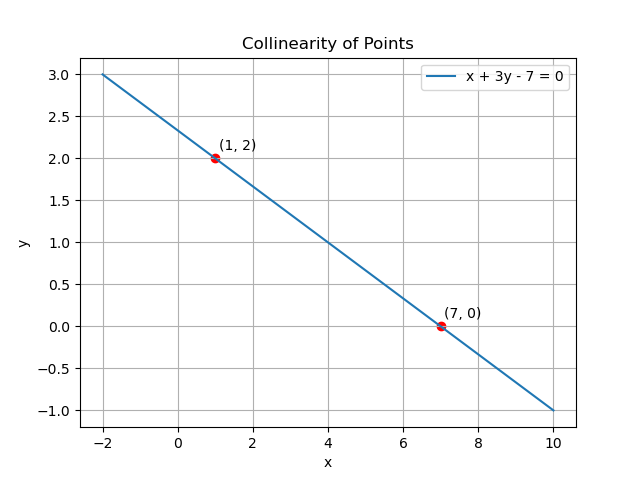
\includegraphics[width=0.7\columnwidth]{figs/fig1.png}
\caption{}
\label{}
\end{figure}

\end{document}
